% Appendix Template

\chapter{DeSIRe: Deep Signer-Invariant Representations for Sign Language Recognition -- supplementary material} % Main appendix title
\chaptermark{DeSIRe -- supplementary material}

\label{appendix:desire} % Change X to a consecutive letter; for referencing this appendix elsewhere, use \ref{AppendixX}

\section{Architecture}
\label{sec:desire_arch}
As shown in \Figref{fig:desire_arch}, the architecture of DeSIRe comprises a CVAE and a classifier.


\begin{figure*}[t]
    \tikzset{every picture/.style={line width=0.75pt}} %set default line width to 0.75pt
    \resizebox{\linewidth}{!}{

        \tikzset{every picture/.style={line width=0.75pt}} %set default line width to 0.75pt

        \begin{tikzpicture}[x=0.75pt,y=0.75pt,yscale=-1,xscale=1]
            %uncomment if require: \path (0,553.8125); %set diagram left start at 0, and has height of 553.8125

            %Shape: Rectangle [id:dp9668838668854731]
            \draw  [draw opacity=0][fill={rgb, 255:red, 155; green, 155; blue, 155 }  ,fill opacity=0.18 ] (39.96,83) -- (583.3,83) -- (583.3,379) -- (39.96,379) -- cycle ;
            %Shape: Rectangle [id:dp2870131986729907]
            \draw  [draw opacity=0][fill={rgb, 255:red, 94; green, 94; blue, 227 }  ,fill opacity=0.21 ] (592.3,104.2) -- (765.3,104.2) -- (765.3,306.2) -- (592.3,306.2) -- cycle ;
            %Shape: Trapezoid [id:dp13927943400330056]
            \draw   (253.96,358) -- (270.46,303) -- (388,303) -- (404.5,358) -- cycle ;
            %Straight Lines [id:da08106004131602051]
            \draw    (276.5,389.81) -- (276.5,360.81) ;
            \draw [shift={(276.5,358.81)}, rotate = 450] [fill={rgb, 255:red, 0; green, 0; blue, 0 }  ][line width=0.75]  [draw opacity=0] (8.93,-4.29) -- (0,0) -- (8.93,4.29) -- cycle    ;

            %Straight Lines [id:da524881694315509]
            \draw    (329.5,389.81) -- (329.5,360.81) ;
            \draw [shift={(329.5,358.81)}, rotate = 450] [fill={rgb, 255:red, 0; green, 0; blue, 0 }  ][line width=0.75]  [draw opacity=0] (8.93,-4.29) -- (0,0) -- (8.93,4.29) -- cycle    ;

            %Straight Lines [id:da32132034584597524]
            \draw    (387.5,389.81) -- (387.5,360.81) ;
            \draw [shift={(387.5,358.81)}, rotate = 450] [fill={rgb, 255:red, 0; green, 0; blue, 0 }  ][line width=0.75]  [draw opacity=0] (8.93,-4.29) -- (0,0) -- (8.93,4.29) -- cycle    ;

            %Shape: Rectangle [id:dp25619693812681654]
            \draw   (261.96,263) -- (323.5,263) -- (323.5,282) -- (261.96,282) -- cycle ;
            %Shape: Rectangle [id:dp6561097472956672]
            \draw   (335.96,263) -- (397.5,263) -- (397.5,282) -- (335.96,282) -- cycle ;
            %Straight Lines [id:da3297304820197924]
            \draw    (292.96,303) -- (292.96,284) ;
            \draw [shift={(292.96,282)}, rotate = 450] [fill={rgb, 255:red, 0; green, 0; blue, 0 }  ][line width=0.75]  [draw opacity=0] (8.93,-4.29) -- (0,0) -- (8.93,4.29) -- cycle    ;

            %Straight Lines [id:da9909219929881732]
            \draw    (365.96,303) -- (365.96,284) ;
            \draw [shift={(365.96,282)}, rotate = 450] [fill={rgb, 255:red, 0; green, 0; blue, 0 }  ][line width=0.75]  [draw opacity=0] (8.93,-4.29) -- (0,0) -- (8.93,4.29) -- cycle    ;

            %Shape: Rectangle [id:dp9663782521635895]
            \draw   (296.96,190) -- (358.5,190) -- (358.5,209) -- (296.96,209) -- cycle ;
            %Straight Lines [id:da590946690938895]
            \draw    (327.89,233.33) -- (328.12,211.59) ;
            \draw [shift={(328.14,209.59)}, rotate = 450.61] [fill={rgb, 255:red, 0; green, 0; blue, 0 }  ][line width=0.75]  [draw opacity=0] (8.93,-4.29) -- (0,0) -- (8.93,4.29) -- cycle    ;

            %Straight Lines [id:da07722147439481009]
            \draw    (292.63,262.69) -- (292.5,237.15) -- (320.5,237.15) ;
            \draw [shift={(322.5,237.15)}, rotate = 180] [fill={rgb, 255:red, 0; green, 0; blue, 0 }  ][line width=0.75]  [draw opacity=0] (8.93,-4.29) -- (0,0) -- (8.93,4.29) -- cycle    ;

            %Straight Lines [id:da9195914844324597]
            \draw    (365.3,263) -- (365.3,244) ;
            \draw [shift={(365.3,242)}, rotate = 450] [fill={rgb, 255:red, 0; green, 0; blue, 0 }  ][line width=0.75]  [draw opacity=0] (8.93,-4.29) -- (0,0) -- (8.93,4.29) -- cycle    ;

            %Straight Lines [id:da3560337897063812]
            \draw    (359.97,237.02) -- (335,237.2) ;
            \draw [shift={(333,237.22)}, rotate = 359.58000000000004] [fill={rgb, 255:red, 0; green, 0; blue, 0 }  ][line width=0.75]  [draw opacity=0] (8.93,-4.29) -- (0,0) -- (8.93,4.29) -- cycle    ;

            %Shape: Trapezoid [id:dp5240821509791835]
            \draw   (402.64,112.89) -- (385.86,167.8) -- (268.32,167.19) -- (252.11,112.11) -- cycle ;
            %Straight Lines [id:da7057163615555322]
            \draw    (326.96,189.5) -- (327.07,169.86) ;
            \draw [shift={(327.08,167.86)}, rotate = 450.31] [fill={rgb, 255:red, 0; green, 0; blue, 0 }  ][line width=0.75]  [draw opacity=0] (8.93,-4.29) -- (0,0) -- (8.93,4.29) -- cycle    ;

            %Straight Lines [id:da5906450135495729]
            \draw    (389.3,182.2) -- (366.3,182.2) -- (366.11,170.06) ;
            \draw [shift={(366.08,168.06)}, rotate = 449.11] [fill={rgb, 255:red, 0; green, 0; blue, 0 }  ][line width=0.75]  [draw opacity=0] (8.93,-4.29) -- (0,0) -- (8.93,4.29) -- cycle    ;

            %Straight Lines [id:da025930072098421686]
            \draw    (403.5,237.15) -- (371.63,237.03) ;
            \draw [shift={(369.63,237.02)}, rotate = 360.21000000000004] [fill={rgb, 255:red, 0; green, 0; blue, 0 }  ][line width=0.75]  [draw opacity=0] (8.93,-4.29) -- (0,0) -- (8.93,4.29) -- cycle    ;

            %Shape: Rectangle [id:dp4487156975269353]
            \draw   (642.15,190) -- (719.15,190) -- (719.15,209) -- (642.15,209) -- cycle ;
            %Straight Lines [id:da726408181609485]
            \draw    (679.96,230) -- (679.96,211) ;
            \draw [shift={(679.96,209)}, rotate = 450] [fill={rgb, 255:red, 0; green, 0; blue, 0 }  ][line width=0.75]  [draw opacity=0] (8.93,-4.29) -- (0,0) -- (8.93,4.29) -- cycle    ;

            %Straight Lines [id:da03770122050678193]
            \draw    (678.96,189.5) -- (678.96,170.5) ;
            \draw [shift={(678.96,168.5)}, rotate = 450] [fill={rgb, 255:red, 0; green, 0; blue, 0 }  ][line width=0.75]  [draw opacity=0] (8.93,-4.29) -- (0,0) -- (8.93,4.29) -- cycle    ;

            %Rounded Rect [id:dp3917167881440844]
            \draw  [color={rgb, 255:red, 208; green, 2; blue, 27 }  ,draw opacity=1 ][dash pattern={on 4.5pt off 4.5pt}] (488.96,193.48) .. controls (488.96,191.27) and (490.75,189.48) .. (492.96,189.48) -- (568.5,189.48) .. controls (570.71,189.48) and (572.5,191.27) .. (572.5,193.48) -- (572.5,205.48) .. controls (572.5,207.69) and (570.71,209.48) .. (568.5,209.48) -- (492.96,209.48) .. controls (490.75,209.48) and (488.96,207.69) .. (488.96,205.48) -- cycle ;
            %Shape: Trapezoid [id:dp14994216757081924]
            \draw   (50.96,358) -- (67.46,303) -- (185,303) -- (201.5,358) -- cycle ;
            %Straight Lines [id:da5750242233036462]
            \draw    (73.5,389.81) -- (73.5,360.81) ;
            \draw [shift={(73.5,358.81)}, rotate = 450] [fill={rgb, 255:red, 0; green, 0; blue, 0 }  ][line width=0.75]  [draw opacity=0] (8.93,-4.29) -- (0,0) -- (8.93,4.29) -- cycle    ;

            %Straight Lines [id:da4377938235507963]
            \draw    (126.5,389.81) -- (126.5,360.81) ;
            \draw [shift={(126.5,358.81)}, rotate = 450] [fill={rgb, 255:red, 0; green, 0; blue, 0 }  ][line width=0.75]  [draw opacity=0] (8.93,-4.29) -- (0,0) -- (8.93,4.29) -- cycle    ;

            %Straight Lines [id:da8126089810991599]
            \draw    (184.5,389.81) -- (184.5,360.81) ;
            \draw [shift={(184.5,358.81)}, rotate = 450] [fill={rgb, 255:red, 0; green, 0; blue, 0 }  ][line width=0.75]  [draw opacity=0] (8.93,-4.29) -- (0,0) -- (8.93,4.29) -- cycle    ;

            %Shape: Rectangle [id:dp9653391052056823]
            \draw   (58.96,263) -- (120.5,263) -- (120.5,282) -- (58.96,282) -- cycle ;
            %Shape: Rectangle [id:dp4596105006317668]
            \draw   (132.96,263) -- (194.5,263) -- (194.5,282) -- (132.96,282) -- cycle ;
            %Straight Lines [id:da6809845179600347]
            \draw    (89.96,303) -- (89.96,284) ;
            \draw [shift={(89.96,282)}, rotate = 450] [fill={rgb, 255:red, 0; green, 0; blue, 0 }  ][line width=0.75]  [draw opacity=0] (8.93,-4.29) -- (0,0) -- (8.93,4.29) -- cycle    ;

            %Straight Lines [id:da05742226043250653]
            \draw    (162.96,303) -- (162.96,284) ;
            \draw [shift={(162.96,282)}, rotate = 450] [fill={rgb, 255:red, 0; green, 0; blue, 0 }  ][line width=0.75]  [draw opacity=0] (8.93,-4.29) -- (0,0) -- (8.93,4.29) -- cycle    ;

            %Straight Lines [id:da4548772108122534]
            \draw [color={rgb, 255:red, 0; green, 0; blue, 0 }  ,draw opacity=1 ]   (212.2,329.57) .. controls (213.87,327.9) and (215.53,327.9) .. (217.2,329.57) .. controls (218.87,331.24) and (220.53,331.24) .. (222.2,329.57) .. controls (223.87,327.9) and (225.53,327.9) .. (227.2,329.57) .. controls (228.87,331.24) and (230.53,331.24) .. (232.2,329.57) .. controls (233.87,327.9) and (235.53,327.9) .. (237.2,329.57) .. controls (238.87,331.24) and (240.53,331.24) .. (242.2,329.57) -- (242.87,329.57) -- (242.87,329.57)(212.2,332.57) .. controls (213.87,330.9) and (215.53,330.9) .. (217.2,332.57) .. controls (218.87,334.24) and (220.53,334.24) .. (222.2,332.57) .. controls (223.87,330.9) and (225.53,330.9) .. (227.2,332.57) .. controls (228.87,334.24) and (230.53,334.24) .. (232.2,332.57) .. controls (233.87,330.9) and (235.53,330.9) .. (237.2,332.57) .. controls (238.87,334.24) and (240.53,334.24) .. (242.2,332.57) -- (242.87,332.57) -- (242.87,332.57) ;


            %Straight Lines [id:da29722450025753333]
            \draw [color={rgb, 255:red, 208; green, 2; blue, 27 }  ,draw opacity=1 ] [dash pattern={on 4.5pt off 4.5pt}]  (358.67,199.31) -- (486.75,199.22) ;
            \draw [shift={(488.75,199.22)}, rotate = 539.96] [fill={rgb, 255:red, 208; green, 2; blue, 27 }  ,fill opacity=1 ][line width=0.75]  [draw opacity=0] (8.93,-4.29) -- (0,0) -- (8.93,4.29) -- cycle    ;

            %Straight Lines [id:da9095959836935932]
            \draw [color={rgb, 255:red, 208; green, 2; blue, 27 }  ,draw opacity=1 ] [dash pattern={on 4.5pt off 4.5pt}]  (575.25,199.32) -- (642.15,199.4) ;

            \draw [shift={(573.25,199.31)}, rotate = 0.07] [fill={rgb, 255:red, 208; green, 2; blue, 27 }  ,fill opacity=1 ][line width=0.75]  [draw opacity=0] (8.93,-4.29) -- (0,0) -- (8.93,4.29) -- cycle    ;
            %Shape: Trapezoid [id:dp5518788435825255]
            \draw   (604.96,285) -- (621.46,230) -- (739,230) -- (755.5,285) -- cycle ;
            %Straight Lines [id:da34976288253592336]
            \draw    (680.5,316.81) -- (680.5,287.81) ;
            \draw [shift={(680.5,285.81)}, rotate = 450] [fill={rgb, 255:red, 0; green, 0; blue, 0 }  ][line width=0.75]  [draw opacity=0] (8.93,-4.29) -- (0,0) -- (8.93,4.29) -- cycle    ;

            %Rounded Rect [id:dp29426784394973304]
            \draw  [color={rgb, 255:red, 208; green, 2; blue, 27 }  ,draw opacity=1 ][dash pattern={on 4.5pt off 4.5pt}] (637.96,67.48) .. controls (637.96,65.27) and (639.75,63.48) .. (641.96,63.48) -- (717.5,63.48) .. controls (719.71,63.48) and (721.5,65.27) .. (721.5,67.48) -- (721.5,79.48) .. controls (721.5,81.69) and (719.71,83.48) .. (717.5,83.48) -- (641.96,83.48) .. controls (639.75,83.48) and (637.96,81.69) .. (637.96,79.48) -- cycle ;
            %Shape: Rectangle [id:dp5888244148515187]
            \draw   (641.3,129.67) -- (718.87,129.67) -- (718.87,169) -- (641.3,169) -- cycle ;
            %Straight Lines [id:da5575811431994107]
            \draw [color={rgb, 255:red, 208; green, 2; blue, 27 }  ,draw opacity=1 ] [dash pattern={on 4.5pt off 4.5pt}]  (677.65,129.5) -- (677.27,86.31) ;
            \draw [shift={(677.25,84.31)}, rotate = 449.49] [fill={rgb, 255:red, 208; green, 2; blue, 27 }  ,fill opacity=1 ][line width=0.75]  [draw opacity=0] (8.93,-4.29) -- (0,0) -- (8.93,4.29) -- cycle    ;

            %Rounded Rect [id:dp027284685274387765]
            \draw  [color={rgb, 255:red, 208; green, 2; blue, 27 }  ,draw opacity=1 ][dash pattern={on 4.5pt off 4.5pt}] (283.96,50.48) .. controls (283.96,48.27) and (285.75,46.48) .. (287.96,46.48) -- (363.5,46.48) .. controls (365.71,46.48) and (367.5,48.27) .. (367.5,50.48) -- (367.5,62.48) .. controls (367.5,64.69) and (365.71,66.48) .. (363.5,66.48) -- (287.96,66.48) .. controls (285.75,66.48) and (283.96,64.69) .. (283.96,62.48) -- cycle ;
            %Straight Lines [id:da8110106070253695]
            \draw [color={rgb, 255:red, 208; green, 2; blue, 27 }  ,draw opacity=1 ] [dash pattern={on 4.5pt off 4.5pt}]  (323.15,112) -- (323.25,69.31) ;
            \draw [shift={(323.25,67.31)}, rotate = 450.13] [fill={rgb, 255:red, 208; green, 2; blue, 27 }  ,fill opacity=1 ][line width=0.75]  [draw opacity=0] (8.93,-4.29) -- (0,0) -- (8.93,4.29) -- cycle    ;

            %Straight Lines [id:da5826581714747092]
            \draw [color={rgb, 255:red, 208; green, 2; blue, 27 }  ,draw opacity=1 ] [dash pattern={on 4.5pt off 4.5pt}]  (397.45,272.7) -- (491.56,272.19) -- (491.56,281.69) ;
            \draw [shift={(491.56,283.69)}, rotate = 270] [fill={rgb, 255:red, 208; green, 2; blue, 27 }  ,fill opacity=1 ][line width=0.75]  [draw opacity=0] (8.93,-4.29) -- (0,0) -- (8.93,4.29) -- cycle    ;

            %Straight Lines [id:da9765435443941437]
            \draw [color={rgb, 255:red, 208; green, 2; blue, 27 }  ,draw opacity=1 ] [dash pattern={on 4.5pt off 4.5pt}]  (311.16,281.68) -- (311.16,297.48) -- (446.96,296.82) ;
            \draw [shift={(448.96,296.81)}, rotate = 539.72] [fill={rgb, 255:red, 208; green, 2; blue, 27 }  ,fill opacity=1 ][line width=0.75]  [draw opacity=0] (8.93,-4.29) -- (0,0) -- (8.93,4.29) -- cycle    ;

            %Rounded Rect [id:dp08457917031260576]
            \draw  [color={rgb, 255:red, 208; green, 2; blue, 27 }  ,draw opacity=1 ][dash pattern={on 4.5pt off 4.5pt}] (75,193) .. controls (75,190.24) and (77.24,188) .. (80,188) -- (219,188) .. controls (221.76,188) and (224,190.24) .. (224,193) -- (224,208) .. controls (224,210.76) and (221.76,213) .. (219,213) -- (80,213) .. controls (77.24,213) and (75,210.76) .. (75,208) -- cycle ;
            %Straight Lines [id:da5903339012593731]
            \draw [color={rgb, 255:red, 208; green, 2; blue, 27 }  ,draw opacity=1 ] [dash pattern={on 4.5pt off 4.5pt}]  (89.95,215.79) -- (89.73,262.63) ;

            \draw [shift={(89.96,213.79)}, rotate = 90.27] [fill={rgb, 255:red, 208; green, 2; blue, 27 }  ,fill opacity=1 ][line width=0.75]  [draw opacity=0] (8.93,-4.29) -- (0,0) -- (8.93,4.29) -- cycle    ;
            %Straight Lines [id:da13585719147268382]
            \draw [color={rgb, 255:red, 208; green, 2; blue, 27 }  ,draw opacity=1 ] [dash pattern={on 4.5pt off 4.5pt}]  (162.81,215.5) -- (162.59,262.34) ;

            \draw [shift={(162.82,213.5)}, rotate = 90.27] [fill={rgb, 255:red, 208; green, 2; blue, 27 }  ,fill opacity=1 ][line width=0.75]  [draw opacity=0] (8.93,-4.29) -- (0,0) -- (8.93,4.29) -- cycle    ;
            %Straight Lines [id:da25575212399218983]
            \draw [color={rgb, 255:red, 208; green, 2; blue, 27 }  ,draw opacity=1 ] [dash pattern={on 4.5pt off 4.5pt}]  (261.32,272.59) -- (199.32,272.5) -- (199.71,215.7) ;
            \draw [shift={(199.72,213.7)}, rotate = 450.39] [fill={rgb, 255:red, 208; green, 2; blue, 27 }  ,fill opacity=1 ][line width=0.75]  [draw opacity=0] (8.93,-4.29) -- (0,0) -- (8.93,4.29) -- cycle    ;

            %Straight Lines [id:da9001250866017318]
            \draw [color={rgb, 255:red, 208; green, 2; blue, 27 }  ,draw opacity=1 ] [dash pattern={on 4.5pt off 4.5pt}]  (346.52,262.5) -- (346.52,254.5) -- (209.32,254.53) -- (209.89,215.88) ;
            \draw [shift={(209.92,213.88)}, rotate = 450.84] [fill={rgb, 255:red, 208; green, 2; blue, 27 }  ,fill opacity=1 ][line width=0.75]  [draw opacity=0] (8.93,-4.29) -- (0,0) -- (8.93,4.29) -- cycle    ;

            %Rounded Rect [id:dp8761394913899854]
            \draw  [color={rgb, 255:red, 208; green, 2; blue, 27 }  ,draw opacity=1 ][dash pattern={on 4.5pt off 4.5pt}] (449.96,290.48) .. controls (449.96,288.27) and (451.75,286.48) .. (453.96,286.48) -- (529.5,286.48) .. controls (531.71,286.48) and (533.5,288.27) .. (533.5,290.48) -- (533.5,302.48) .. controls (533.5,304.69) and (531.71,306.48) .. (529.5,306.48) -- (453.96,306.48) .. controls (451.75,306.48) and (449.96,304.69) .. (449.96,302.48) -- cycle ;
            %Straight Lines [id:da7496006991926858]
            \draw [color={rgb, 255:red, 208; green, 2; blue, 27 }  ,draw opacity=1 ] [dash pattern={on 4.5pt off 4.5pt}]  (750.33,73.21) -- (723,73.21) ;
            \draw [shift={(721,73.21)}, rotate = 360] [fill={rgb, 255:red, 208; green, 2; blue, 27 }  ,fill opacity=1 ][line width=0.75]  [draw opacity=0] (8.93,-4.29) -- (0,0) -- (8.93,4.29) -- cycle    ;

            %Straight Lines [id:da5079252315343075]
            \draw [color={rgb, 255:red, 208; green, 2; blue, 27 }  ,draw opacity=1 ] [dash pattern={on 4.5pt off 4.5pt}]  (397.33,56.21) -- (370,56.21) ;
            \draw [shift={(368,56.21)}, rotate = 360] [fill={rgb, 255:red, 208; green, 2; blue, 27 }  ,fill opacity=1 ][line width=0.75]  [draw opacity=0] (8.93,-4.29) -- (0,0) -- (8.93,4.29) -- cycle    ;


            % Text Node
            \draw (331,318) node  [align=left] {{\footnotesize Encoder:}};
            % Text Node
            \draw (279,408) node   {$\boldsymbol{X}^{r_{i}}_{y_{i} ,\ s_{i}}$};
            % Text Node
            \draw (331,405) node   {$y_{i}$};
            % Text Node
            \draw (388,405) node   {$s_{i}$};
            % Text Node
            \draw (328.23,339.91) node   {$q(\mathbf{z} \mid \mathbf{X}\mathrm{,y,s;}\vtheta _{e})$};
            % Text Node
            \draw (328,237) node   {${\displaystyle \mathbf{\oplus }}$};
            % Text Node
            \draw (366.73,272.5) node   {$2\log \vsigma^{(i)}$};
            % Text Node
            \draw (328.73,199) node   {$\boldsymbol{z}_{i}$};
            % Text Node
            \draw (326,125) node  [align=left] {{\footnotesize Decoder:}};
            % Text Node
            \draw (434,180) node   {$\mathnormal{s_{j} \sim w(}\mathrm{s} \mid \mathnormal{s_{i})}$};
            % Text Node
            \draw (445,235) node   {$\epsilon _{i} \sim \mathcal{N}\mathrm{(} 0,\mathbf{I}\mathrm{)}$};
            % Text Node
            \draw (679.73,199.5) node   {$\tilde{z}_{i}$};
            % Text Node
            \draw (529.73,198.5) node   {${\textstyle \mathcal{\textcolor[rgb]{0.82,0.01,0.11}{L}}\textcolor[rgb]{0.82,0.01,0.11}{_{\text{emb}}}}$};
            % Text Node
            \draw (128,318) node  [align=left] {{\footnotesize Encoder:}};
            % Text Node
            \draw (89.73,272) node   {$\vmu^{(u)}$};
            % Text Node
            \draw (163.73,272) node   {$2\log \vsigma^{(u)}$};
            % Text Node
            \draw (682,245) node  [align=left] {{\footnotesize CNN feature extractor:}};
            % Text Node
            \draw (678.23,265.91) node   {$\mathnormal{g}(\mathbf{X}\mathrm{;}\vtheta _{g})$};
            % Text Node
            \draw (678.73,72.5) node   {${\textstyle \mathcal{\textcolor[rgb]{0.82,0.01,0.11}{L}}\textcolor[rgb]{0.82,0.01,0.11}{_{\text{class}}}}$};
            % Text Node
            \draw (687.33,113.5) node   {$\hat{\mathnormal{y}}_{i}$};
            % Text Node
            \draw (324.73,55.5) node   {${\textstyle \mathcal{\textcolor[rgb]{0.82,0.01,0.11}{L}}\textcolor[rgb]{0.82,0.01,0.11}{_{\text{rec}}}}$};
            % Text Node
            \draw (371.33,98.5) node   {$\boldsymbol{\mu }_{d}(\boldsymbol{z}_{i} ,s_{j} ;\vtheta _{d})$};
            % Text Node
            \draw (680.08,142.67) node  [align=left] {{\footnotesize MLP:}};
            % Text Node
            \draw (680.9,157.57) node   {$g(\tilde{\vz};\vtheta _{g})$};
            % Text Node
            \draw (117.96,438) node [scale=0.9]  {$\mathnormal{y_{\mathnormal{u}} =y_{\mathnormal{i}} ,\ s_{\mathnormal{u}} \neq s_{\mathnormal{i}}}$};
            % Text Node
            \draw (625,114) node  [align=left] {{\footnotesize \textbf{Classifier}}};
            % Text Node
            \draw (86.96,97) node  [align=left] {{\footnotesize \textbf{CVAE \ \ \ \ \ \ \ \ \ \ \ \ \ }}};
            % Text Node
            \draw (77,408) node   {$\boldsymbol{X}^{r_{u}}_{y_{u} ,\ s_{u}}$};
            % Text Node
            \draw (129,405) node   {$y_{u}$};
            % Text Node
            \draw (186,405) node   {$s_{u}$};
            % Text Node
            \draw (681,335) node   {$\boldsymbol{X}^{r_{i}}_{y_{i} ,\ s_{i}}$};
            % Text Node
            \draw (126.23,339.91) node   {$q(\mathbf{z} \mid \mathbf{X}\mathrm{,y,s;}\vtheta _{e})$};
            % Text Node
            \draw (327.23,147.91) node   {$p(\mathbf{X} \mid \mathbf{z}\mathrm{,s;} \vtheta _{d})$};
            % Text Node
            \draw (148,200.5) node   {${\textstyle \mathcal{\textcolor[rgb]{0.82,0.01,0.11}{L}}\textcolor[rgb]{0.82,0.01,0.11}{_{\text{signer\_inv}}}}$};
            % Text Node
            \draw (491.73,296.48) node   {${\textstyle \mathcal{\textcolor[rgb]{0.82,0.01,0.11}{L}}\textcolor[rgb]{0.82,0.01,0.11}{_{\text{prior}}}}$};
            % Text Node
            \draw (292.73,272.5) node   {$\vmu^{(i)}$};
            % Text Node
            \draw (763,73.17) node   {$y_{i}$};
            % Text Node
            \draw (422,58) node   {$\boldsymbol{X}^{r_{j}}_{y_{j} ,\ s_{j}}$};
            % Text Node
            \draw (495.96,61) node [scale=0.9]  {$\mathnormal{y_{j} = y_{\mathnormal{i}}}$};
            % Text Node
            \draw (364.97,237.02) node   {$\mathbf{\odot }$};


        \end{tikzpicture}

    }
    \caption{The architecture of the proposed DeSIRe deep neural network for signer-independent SLR. It comprises two main modules or components: a conditional variational atoencoder (CVAE) and a classifier.}
    \label{fig:desire_arch}
\end{figure*}


\subsection{CVAE}
The CVAE consists of an encoder and a decoder. The encoder network attempts to learn a stochastic mapping from an input image $\mX$, its class label $y$, and signer identity $s$ to a latent representation $\vz$. We condition the encoder on $y$ and $s$ by simply concatenating the class and signer identity as extra channels in the input image. In this case, both $y$ and $s$ are represented categorically using one-hot encoding. The encoder network then consists of a sequence of several $3\times 3$ convolutional layers with batch-normalization and leaky rectified linear units (LeakyReLUs) as non-linearities. For downsampling, the stride length of every convolution is set to 2. On top of that, there are two output fully connected (a.k.a.\ dense) layers, with linear activation functions, describing the mean $\vmu_e(\rmX,\ry,\rs; \vtheta_e)$ and the log-variance $\log \vsigma_e^2(\rmX,\ry,\rs; \vtheta_e)$ of the latent space distribution $q(\rvz \mid \rmX, \ry, \rs; \vtheta_e)$.

The decoder module will then generate a latent code $\vz$ sampled from $q(\rvz \mid \mX, y, s; \vtheta_e)$ and proceed to the reconstruction of the original input $\mX$. In practice, the latent code $\vz$ is concatenated with a one-hot representation of the signer identity $s$ to be fed to the decoder network. The decoder network comprises several 2-D transposed convolutions for up-sampling and densifying the incoming activations. Every transposed convolutional layer is followed by batch-normalization and a LeakyReLU. The output layer also consists of a transposed convolutional layer but with a hyperbolic tangent activation function in order to output the reconstruction $\vmu_d(\vz,s; \vtheta_d)$ of the normalized input $\mX$.

\subsection{Classifier}
The implemented classifier module follows a typical CNN architecture for classification tasks. It starts with a block of convolutional layers for feature extraction purposes, producing representations $\tilde{\vz} \triangleq g(\mX;\vtheta_g)$. This is followed by a block of fully-connected layers for sign classification, which predicts the sign class $\hat{y} \triangleq h(\tilde{\vz};\vtheta_h)$. In particular, the convolutional block comprises a sequence of several pairs of consecutive $3 \times 3$ convolutional layers with ReLUs as non-linearities. For downsampling, the last convolutional layer of each pair has a stride of 2.

The fully-connected block consists of a sequence of fully-connected layers with ReLUs as the non-linear functions. The last fully-connected layer has a softmax activation function which outputs the probabilities for each sign class.

\section{Training strategies}
\label{sec:desire_training_strat}

We have observed experimentally that the classification task is much easier than the reconstruction task of the CVAE. That is, the classifier tends to overfit the data with fewer training epochs than the CVAE, learning embeddings that are essentially not signer-invariant. In order to avoid this behavior, we have adopted an annealing strategy to define the classification weight $\lambda_2$. Specifically, at the start of training, this weight is set to zero, so that the CVAE learns to produce signer-invariant latent representations. At this stage, the CVAE behaves as a pure teacher model for the classifier network and, therefore, the $L_\text{emb}$ error is backpropagated only through the classifier. After a few epochs, the weight $\lambda_2$ starts increasing according to a sigmoid annealing schedule and the $L_\text{emb}$ loss starts to be backpropagated through the CVAE encoder as well. This procedure will endow the CVAE with a better sense of the classification task and hence promote class separability in the latent space. As a result, the model will be able to learn signer-invariant representations that are in fact highly discriminative for the sign recognition task.

Following \citet{Bowman2015} and in order to stabilize the training of the CVAE, we have employed a similar annealing strategy to define the KL divergence weights of the prior and signer-invariant loss terms, $\alpha_1$ and $\alpha_2$, respectively.

\section{Implementation details}
All deep models were implemented in PyTorch and trained with the Adam optimization algorithm using a batch size of 32 samples. For reproducibility purposes, the source code as well as the weights of the trained models are publicly available online\footnote{URL will be made available after the decision.}.

The hyperparameters that are common to all the implemented models (i.e., the learning rate and the $\normltwo$ regularization coefficient) as well as some hyperparameters that are specific to the DeSIRe model (i.e.\ $\lambda_{1}$, $\lambda_{2}$, $\alpha_{1}$ and $\alpha_{2}$) and to the implemented baseline 2 (i.e.\ $\gamma$) were optimized by means of a grid search approach and cross-validation on the training set. The hyperparameter $\rho$ in $w(\rs \mid s_{i})$, defined for the proposed sampling scheme of the signer identity, was set to $\rho=0.5$. The dropout rate was empirically set at 0.5 for all the experiments. The set of values of the adopted hyperparameters grid search is presented in \Tableref{tab:desire_hyperparam}.

During the training stage of all the implemented models, besides $\normltwo$ regularization and dropout, a randomized data augmentation scheme was also employed. Following \citet{Ferreira2018}, the adopted data augmentation procedure is based on both geometric and colour transformations. The underlying idea is to further increase the robustness of the models to the wide range of hand gestures positions, poses, viewing angles as well as to different illumination conditions and contrasts.

\begin{table}[t]
    \centering
        \begin{tabular}{c|c|c}
            Hyperparameters                    & Symbol & Set                \\\hline
            Leaning rate                                & --       & \{$1\text{e}^{-03}$,$1\text{e}^{-04}$\}             \\
            $\ell^2$-norm coefficient                              & --      & \{$1\text{e}^{-04}$,$1\text{e}^{-05}$\}             \\
            $L_{\text{triplet}}$ weight                 & $\gamma$                & \{0.1,0.5,1,5,10\}                  \\
            $L_{\text{emb}}$ weight                 & $\lambda_{1}$                & \{0.1,0.5\}                  \\
            $L_{\text{class}}$ weight                 & $\lambda_{2}$                & \{1,5,10\}                  \\
            $L_{\text{prior}}$ weight                 & $\alpha_{1}$                & \{$5\text{e}^{-03}$, $8\text{e}^{-02}$\}                  \\
            $L_{\text{signer\_inv}}$ weight                 & $\alpha_{2}$                & \{$8\text{e}^{-02}$, $4\text{e}^{-01}$, $8\text{e}^{-01}$\}                  \\
        \end{tabular}
    \caption{Hyperparameter sets for the DeSIRe model and baselines.}
    \label{tab:desire_hyperparam}
\end{table}


A detailed description of the architecture of the proposed model is presented in \Tableref{table:desire_arch}. For illustrative purposes, the presented DeSIRe architecture considers input colour images with a resolution of $100\times 100$ pixels, 10 signer identities in the training set and a total of 10 sign classes. It is important to stress out that, for a fair comparison, the topology of both implemented baselines follows the same architecture of the classifier component of the proposed DeSIRe model.

\begin{table}[t]
    \centering
        \begin{tabular}{c|c|c|c|c|c}
            \begin{tabular}[c]{@{}c@{}}Layer\\ \#\end{tabular} & \begin{tabular}[c]{@{}c@{}}DeSIRe\\ module\end{tabular} &Layer type  & \begin{tabular}[c]{@{}c@{}}Non-\\ linearity\end{tabular} & Output shape & Connected to                                                                    \\ \hline
            -                                                           & \multirow{4}{*}{\rotatebox[origin=c]{90}{Inputs}}                                         & input\_x                                                                           & -                                                                 & (3,100,100)           & -                                                                                        \\
            -                                                           &                                                                 & input\_y\_2d                                                                      & -                                                                 & (10,100,100)          & -                                                                                        \\
            -                                                           &                                                                 & input\_s\_2d                                                                     & -                                                                 & (10,100,100)          & -                                                                                        \\
            -                                                           &                                                                 & input\_s\_1d                                                                       & -                                                                 & (10,)                 & -                                                                                        \\ \hline
            1                                                           & \multirow{9}{*}{\rotatebox[origin=c]{90}{$q(\rvz \mid \rmX, \ry, \rs; \vtheta_e)$}}                                        & Concat2d-1                                                                      & -                                                                 & (23,100,100)          & \begin{tabular}[c]{@{}c@{}}{[}input\_x; \\ input\_y\_2d; \\ input\_s\_2d{]}\end{tabular} \\
            2                                                           &                                                                 & Conv2d-1                                                                         & LeakyReLU                                                         & (64,50,50)            & Concat2d-1                                                                               \\
            3                                                           &                                                                 & Conv2d-2                                                                        & LeakyReLU                                                         & (64,25,25)            & Conv2d-1                                                                                 \\
            4                                                           &                                                                 & Conv2d-3                                                                         & LeakyReLU                                                         & (128,13,13)           & Conv2d-2                                                                                 \\
            5                                                           &                                                                 & Conv2d-4                                                                        & LeakyReLU                                                         & (256,7,7)             & Conv2d-3                                                                                 \\
            6                                                           &                                                                 & Conv2d-5                                                                         & LeakyReLU                                                         & (512,4,4)             & Conv2d-4                                                                                 \\
            7                                                           &                                                                 & Dense-1                                                                          & Linear                                                            & (128,)                & Conv2d-5                                                                                 \\
            8                                                           &                                                                 & Dense-2                                                                        & Linear                                                            & (128,)                & Conv2d-5                                                                                 \\
            9                                                           &                                                                 & Dense-3                                                                         & LeakyReLU                                                         & (128,)                & \begin{tabular}[c]{@{}c@{}}{[}Dense-1; \\ Dense-2{]}\end{tabular}                        \\ \hline
            10                                                          & \multirow{7}{*}{\rotatebox[origin=c]{90}{$p(\rmX \mid \rvz, \rs; \vtheta_d)$}}                                        & Concat1d-1                                                                        & -                                                                 & (138,)                & \begin{tabular}[c]{@{}c@{}}{[}Dense-3; \\ input\_s\_1d{]}\end{tabular}                   \\
            11                                                          &                                                                 & Reshape-1                                                                        & -                                                                 & (512,4,4)             & Concat1d-1                                                                               \\
            12                                                          &                                                                 & ConvTr2d-1                                                               & LeakyReLU                                                         & (512,7,7)             & Reshape-1                                                                                \\
            13                                                          &                                                                 & ConvTr2d-2                                                                & LeakyReLU                                                         & (256,13,13)           & ConvTr2d-1                                                                        \\
            14                                                          &                                                                 & ConvTr2d-3                                                               & LeakyReLU                                                         & (128,25,25)           & ConvTr2d-2                                                                        \\
            15                                                          &                                                                 & ConvTr2d-4                                                                & LeakyReLU                                                         & (64,50,50)            & ConvTr2d-3                                                                        \\
            16                                                          &                                                                 & ConvTr2d-5                                                              & Tanh                                                              & (3,100,100)           & ConvTr2d-4                                                                        \\ \hline
            17                                                          & \multirow{6}{*}{\rotatebox[origin=c]{90}{$g(\mX; \vtheta_g)$}}                                           & Conv2d-6                                                                          & ReLU                                                              & (32,100,100)          & input\_x                                                                                 \\
            18                                                          &                                                                 & Conv2d-7                                                                        & ReLU                                                              & (32,50,50)            & Conv2d-6                                                                                 \\
            19                                                          &                                                                 & Conv2d-8                                                                          & ReLU                                                              & (64,50,50)            & Conv2d-7                                                                                 \\
            20                                                          &                                                                 & Conv2d-9                                                                         & ReLU                                                              & (64,25,25)            & Conv2d-8                                                                                 \\
            21                                                          &                                                                 & Conv2d-19                                                                          & ReLU                                                              & (128,13,13)           & Conv2d-9                                                                                 \\
            22                                                          &                                                                 & Conv2d-11                                                                         & ReLU                                                              & (128,13,13)           & Conv2d-10                                                                                 \\ \hline
            23                                                          & \multirow{5}{*}{\rotatebox[origin=c]{90}{$h(\tilde{\vz}; \vtheta_h)$}}                                          & Dense-4                                                                         & ReLU                                                              & (128,)                & Conv2d-11                                                                                \\
            24                                                          &                                                                 & Dropout-1                                                                         & -                                                                 & (128,)                & Dense-4                                                                                  \\
            25                                                          &                                                                 & Dense-5                                                                           & ReLU                                                              & (128,)                & Dropout-1                                                                                \\
            26                                                          &                                                                 & Dropout-2                                                                          & -                                                                 & (128,)                & Dense-5                                                                                  \\
            27                                                          &                                                                 & Dense-6                                                                          & Softmax                                                              & (10,)                 & Dropout-2                                                                                \\
        \end{tabular}
    \caption{A detailed description of the architecture of the proposed DeSIRe model. The output shape is described as (\#filters, rows, columns).}
    \label{table:desire_arch}
\end{table}

\section{Visualization of the latent space}
\label{sec:desire_tsne}
In this section, we present a 2-D visualization of the learned embedding via t-SNE, similarly to what we have done for our previous adversarial model (\Secref{sec:adv_signer_inv_tsne}).

\Figref{fig:desire_tsne_a} depicts the t-SNE provided by the DeSIRe model and both implemented baselines in two test splits, of the MKLM dataset, with different degrees of inter-signer variability. \Figref{fig:desire_tsne_b} illustrates the t-SNE plots obtained by the domain adaptation methods (DANN and DTML) for the same exact test splits. For easier comparison, we show the results for DeSIRe in both figures.

\begin{figure}[ht!]
    \begin{minipage}[t!]{0.015\textwidth}
        \rotatebox[origin=c]{90}{\footnotesize{Test split 1}}
    \end{minipage}
    \begin{minipage}[t!]{0.985\textwidth}
        \captionsetup[subfigure]{labelformat=empty}
        \centering
        \begin{subfigure}{0.325\textwidth}
            \centering
            \subcaption[short for lof]{CNN (baseline 1)}
            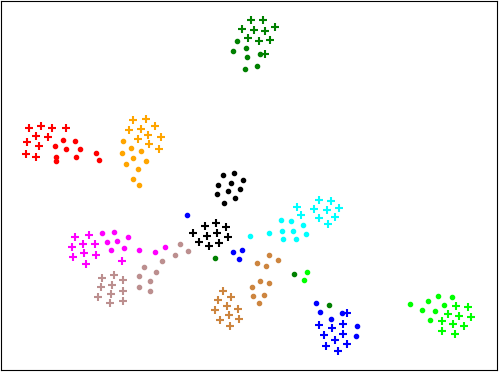
\includegraphics[width=\linewidth]{ChapterFour/cnn_tsne_3.png}
            \caption{accuracy: 95.50 \%}
        \end{subfigure}
        \hfill
        \begin{subfigure}{0.325\textwidth}
            \centering
            \subcaption[short for lof]{CNN with triplet loss (baseline 2)}
            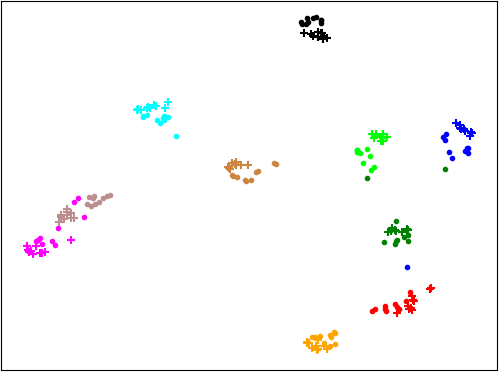
\includegraphics[width=\linewidth]{ChapterFour/triplet_tsne_3.png}
            \caption{accuracy: 96.50 \%}
        \end{subfigure}
        \hfill
        \begin{subfigure}{0.325\textwidth}
            \centering
            \subcaption[short for lof]{DeSIRe}
            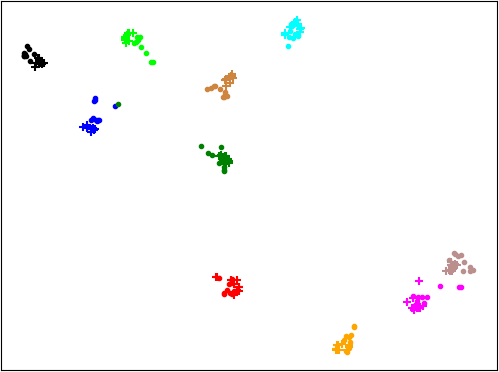
\includegraphics[width=\linewidth]{ChapterFour/desire_tsne_3.png}
            \caption{accuracy: 98.50 \%}
        \end{subfigure}
    \end{minipage}
    \\ \vspace{0.5 cm}
    \begin{minipage}[t!]{0.015\textwidth}
        \rotatebox[origin=c]{90}{\footnotesize{Test split 2}}
    \end{minipage}
    \begin{minipage}[t!]{0.985\textwidth}
        \captionsetup[subfigure]{labelformat=empty}
        \begin{subfigure}{0.325\textwidth}
            \centering
            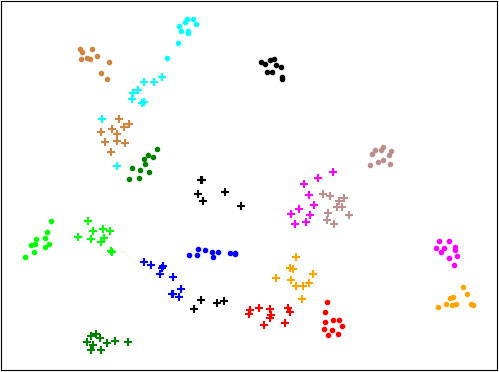
\includegraphics[width=\linewidth]{ChapterFour/cnn_tsne_2.png}
            \caption{accuracy: 73.00 \%}
        \end{subfigure}
        \hfill
        \begin{subfigure}{0.325\textwidth}
            \centering
            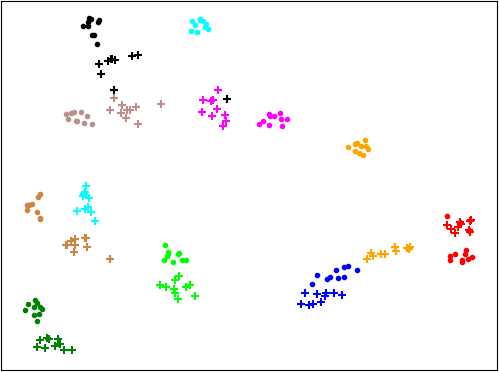
\includegraphics[width=\linewidth]{ChapterFour/triplet_tsne_2.png}
            \caption{accuracy: 86.50 \%}
        \end{subfigure}
        \hfill
        \begin{subfigure}{0.325\textwidth}
            \centering
            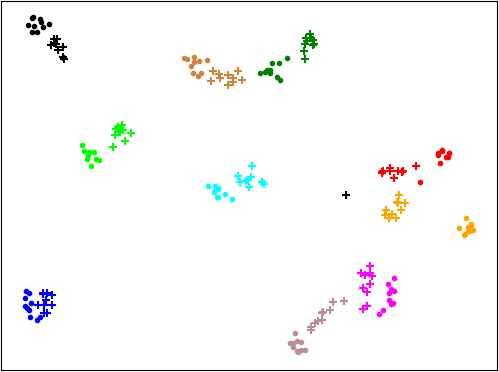
\includegraphics[width=\linewidth]{ChapterFour/desire_tsne_2.png}
            \caption{accuracy: 98.50 \%}
        \end{subfigure}
    \end{minipage}
    \caption{Two-dimensional projection of the latent representation space provided by DeSIRe and both baselines, using t-SNE \cite{Maaten2008}. Markers $\bullet$ and $\textbf{+}$ represent two different test signers from the MKLM dataset and the different colors correspond to the 10 sign classes. The accuracy of each model on each split is shown below each picture.}
    \label{fig:desire_tsne_a}
\end{figure}

As it is possible to observe in Figures~\ref{fig:desire_tsne_a} and \ref{fig:desire_tsne_b}, all the implemented models achieved high classification accuracies on the test split~1. Nevertheless, the t-SNE plots clearly demonstrate the better capability of DeSIRe to impose signer-independence in the latent representations. The DeSIRe model yields a latent representation space in which latent representations of the same signer and different classes are close to each other and well mixed, while it keeps latent representations of different classes far apart.

The test split~2, depicted in the bottom row of Figures~\ref{fig:desire_tsne_a} and \ref{fig:desire_tsne_b}, is characterized by a larger inter-signer variability. Consequently, for this particular test split, the gains of DeSIRe are much more noticeable. Specifically, the DeSIRe model achieved $98.50\%$ classification accuracy against $73.00\%$, $86.50\%$, $91.50\%$ and $87.00\%$ of baseline 1, baseline 2, DANN, and DTML, respectively. The t-SNE plots support these classification results (see the bottom row of Figures~\ref{fig:desire_tsne_a} and \ref{fig:desire_tsne_b}). There, it is possible to observe that baseline 1 completely fails in the arrangement of the latent space. Specifically, the latent representations of different signers and the same class are too far apart. In addition, there is a clear overlap between clusters of different classes. Although the CNN with the triplet loss (i.e.\ baseline 2) and both domain adaptation methods promoted slight improvements over the standard baseline CNN, the proposed DeSIRe model achieved by far the best inter-class separability.

\begin{figure}[ht!]
    \begin{minipage}[t!]{0.015\textwidth}
        \rotatebox[origin=c]{90}{\footnotesize{Test split 1}}
    \end{minipage}
    \begin{minipage}[t!]{0.985\textwidth}
        \captionsetup[subfigure]{labelformat=empty}
        \centering
        \begin{subfigure}{0.325\textwidth}
            \centering
            \subcaption[short for lof]{DANN \cite{Ganin2015}}
            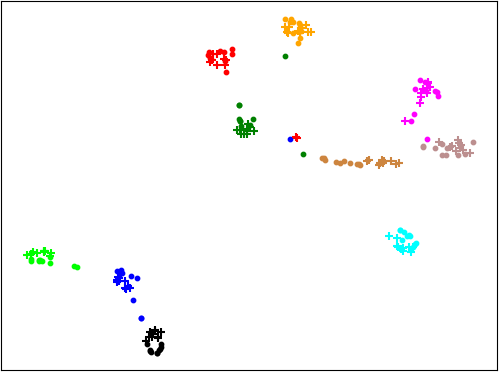
\includegraphics[width=\linewidth]{ChapterFour/ganin_tsne_3.png}
            \caption{accuracy: 95.50 \%}
        \end{subfigure}
        \hfill
        \begin{subfigure}{0.325\textwidth}
            \centering
            \subcaption[short for lof]{DTML \cite{Hu2016}}
            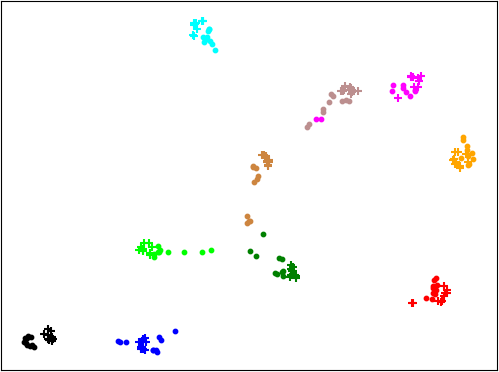
\includegraphics[width=\linewidth]{ChapterFour/hu_tsne_3.png}
            \caption{accuracy: 97.50 \%}
        \end{subfigure}
        \hfill
        \begin{subfigure}{0.325\textwidth}
            \centering
            \subcaption[short for lof]{DeSIRe}
            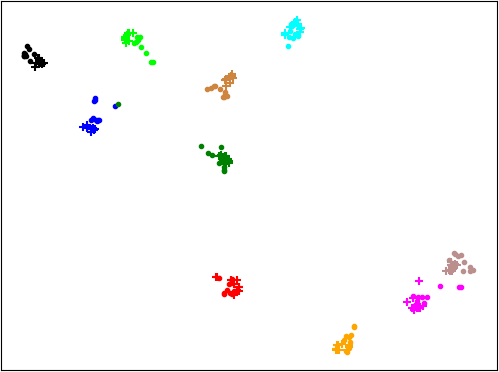
\includegraphics[width=\linewidth]{ChapterFour/desire_tsne_3.png}
            \caption{accuracy: 98.50 \%}
        \end{subfigure}
    \end{minipage}
    \\ \vspace{0.5 cm}
    \begin{minipage}[t!]{0.015\textwidth}
        \rotatebox[origin=c]{90}{\footnotesize{Test split 2}}
    \end{minipage}
    \begin{minipage}[t!]{0.985\textwidth}
        \captionsetup[subfigure]{labelformat=empty}
        \begin{subfigure}{0.325\textwidth}
            \centering
            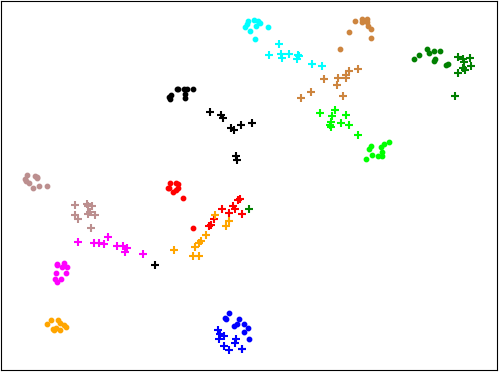
\includegraphics[width=\linewidth]{ChapterFour/ganin_tsne_2.png}
            \caption{accuracy: 91.50 \%}
        \end{subfigure}
        \hfill
        \begin{subfigure}{0.325\textwidth}
            \centering
            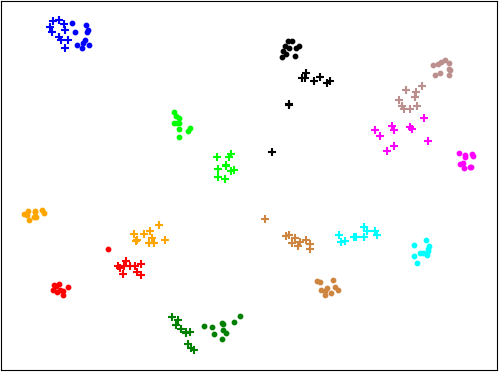
\includegraphics[width=\linewidth]{ChapterFour/hu_tsne_2.png}
            \caption{accuracy: 87.00 \%}
        \end{subfigure}
        \hfill
        \begin{subfigure}{0.325\textwidth}
            \centering
            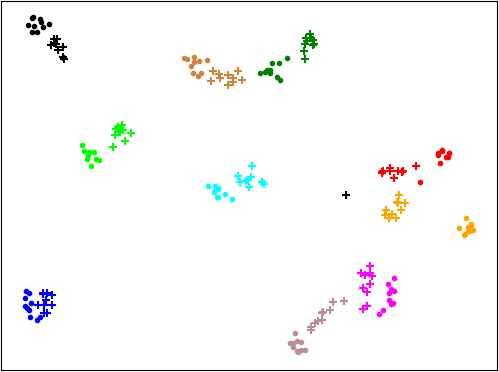
\includegraphics[width=\linewidth]{ChapterFour/desire_tsne_2.png}
            \caption{accuracy: 98.50 \%}
        \end{subfigure}
    \end{minipage}
    \caption{Two-dimensional projection of the latent representation space provided by DeSIRe, DANN, and DTML, using t-SNE \cite{Maaten2008}. Markers $\bullet$ and $\textbf{+}$ represent two different test signers from the MKLM dataset and the different colors correspond to the 10 sign classes. The accuracy of each model on each split is shown below each picture.}
    \label{fig:desire_tsne_b}
\end{figure}

\section{Cluster analysis in the latent space}
\label{sec:desire_clusters}
In order to obtain an objective quality assessment of the produced latent representations, we have evaluated how well the model is able to cluster the different sign classes (and thus ignore the signer identity) in the latent space. For this purpose, we use two cluster validation metrics: the average Silhouette coefficient (\citet{Rousseeuw1987}) per cluster and the Dunn's index (\citet{Dunn1973}) per cluster.

The Silhouette coefficient for an observation $i$ is computed as follows. Let $C_i$ be the cluster (sign class) associated with the observation $i$. The average intra-cluster distance $a_i$ and the minimum average inter-cluster distance $b_i$ for the observation $i$ are obtained as follows:
\begin{align}
    a_i &= \frac{1}{|C_i|-1} \sum_{j \in C_i} d(i,j),\\
    b_i &= \min_{\overline{C} \neq C_i} \frac{1}{|\overline{C}|} \sum_{j \in \overline{C}} d(i,j),
\end{align}
where $|C_i|$ denotes the number of observations in the cluster $|C_i|$ and $d(i,j)$ is the Euclidean distance between the observations $i$ and $j$. Then, the Silhouette index $S_i$ for the observation $i$ is defined as:
\begin{equation}
    S_i = \frac{b_i - a_i}{\max(a_i, b_i)}.
\end{equation}
Clearly, $-1 \leq S_i \leq 1$. Intuitively, clusters are desirably compact (small $a_i$) and well separated (large $b_i$), so a larger value of $S_i$ indicates better clustering. However, this metric is defined per observation. Hence, in order to have a global measure of clustering quality, we compute the average Silhouette coefficient for each cluster.

Dunn's index follows a similar idea of measuring cluster compactness versus separation, but uses minimum and maximum distances instead of average distances, and is more sensitive to extreme and occasional errors. Specifically, Dunn's index $D_C$ for a cluster $C$ is defined as the ratio between the minimum inter-cluster distance $\delta_C$ from $C$ to all other clusters (which measures cluster separation) and the maximum intra-cluster distance $\Delta_C$ for the cluster $C$ (which measures cluster compactness):
\begin{equation}
    \delta_C = \min_{i \in C, j \not\in C} d(i,j), \quad \Delta_C = \max_{i,j \in C} d(i,j), \quad  D_C = \frac{\delta_C}{\Delta_C}.
\end{equation}
Again, according to this metric, larger values indicate better clustering.
Results are shown in \Tableref{tab:signer_inv_metric}. As anticipated by the analysis of the two-dimensional t-SNE projection in Figures~\ref{fig:desire_tsne_a} and \ref{fig:desire_tsne_b}, the results confirm that the DeSIRe model produces the most compact and separated sign clusters, when compared with the remaining models. This observation supports the signer-invariance property of the representations produced by the DeSIRe model: when exposed to images obtained from new signers, our model does a better job of grouping them according to the respective sign class only, ignoring the signer identity. Baseline 2 and DTML are also capable of producing fairly good sign clusters. This is not a surprising fact since both approaches include explicit penalties in the respective training objectives that favor compactness in the latent space among samples of the same sign class. The absence of such a compactness constraint in DANN allows its latent representations to be more widely spread over the latent space. As such, according to the adopted metrics, the obtained sign clusters are comparable to those obtained using a simple CNN (baseline 1), although the resulting sign classification accuracy is undoubtedly superior.

\begin{table}[t]
    \centering
    \resizebox{1\textwidth}{!}{
        \begin{tabular}{c |c c c c|c c c c|c c c c}
            & \multicolumn{4}{c |}{Jochen-Triesch}                                               & \multicolumn{4}{c|}{MKLM}                                                  & \multicolumn{4}{c}{CorSiL}                                                \\
            & \multicolumn{2}{c}{Dunn's} & \multicolumn{2}{c|}{Silhouette} & \multicolumn{2}{c}{Dunn's} & \multicolumn{2}{c|}{Silhouette} & \multicolumn{2}{c}{Dunn's} & \multicolumn{2}{c}{Silhouette} \\
            & Average     & min    & Average     & min    & Average     & min    & Average     & min    & Average     & min    & Average     & min    \\ \hline
            DANN \cite{Ganin2015}                  &   0.165              &    0.105          &       0.457          &       0.342       &    0.380             &      0.102       &       0.531         &      0.253        &          0.310      &       0.205      &       0.281          &       0.109       \\
            DTML \cite{Hu2016}                   &      0.218           &    0.170          &          0.557       &       0.493       &       0.693          &      0.236        &      \textbf{0.653}           &         0.342     &        0.298         &      0.200        &       0.312          &    0.107          \\
            \hline
            CNN (baseline 1)                   & 0.171                & 0.132             & 0.405                & 0.326             & 0.378                & 0.159             & 0.537                & 0.295             & 0.346                & 0.184             & 0.316                & 0.112             \\
            CNN with triplet loss (baseline 2) & 0.249                & 0.179             & 0.509                & 0.453             & 0.559                & 0.208             & 0.623                & 0.171             & 0.359                & \textbf{0.210}    & 0.313                & 0.186             \\
            DeSIRe              & \textbf{0.316}       & \textbf{0.184}    & \textbf{0.582}       & \textbf{0.541}    & \textbf{0.695}       & \textbf{0.240}    & 0.646       & \textbf{0.377}    & \textbf{0.374}       & 0.186             & \textbf{0.320}       & \textbf{0.197}    \\
        \end{tabular}}
        \caption{Dunn's index and Silhouette coefficient for the sign class clusters in the latent space for the test data. These metrics were computed per cluster and the average and minimum results are reported for each model and dataset.}
        \label{tab:signer_inv_metric}
\end{table}


\section{Unveiling the training behavior of DeSIRe}
\label{sec:desire_training_behav}
In this subsection, we further analyze the training process of the proposed DeSIRe model. \Figref{fig:desire_loss_curves} shows the behavior of different loss terms, over 150 epochs of training on the MKLM dataset, with the sigmoid annealing schedules in place. Specifically, we have plotted the curves of the key loss terms, $L_{\text{signer\_inv}}$ and $L_{\text{emb}}$, responsible for promoting signer-invariant latent representations (see Figures~\ref{fig:signer_inv_curve} and \ref{fig:emb_loss_curve}, respectively). In addition, we have also plotted the curve of the classification loss term $L_{\text{class}}$, which trains the model to predict the output sign labels.

\begin{figure}[t]
    \centering
    \begin{subfigure}{0.325\textwidth}
        \centering
        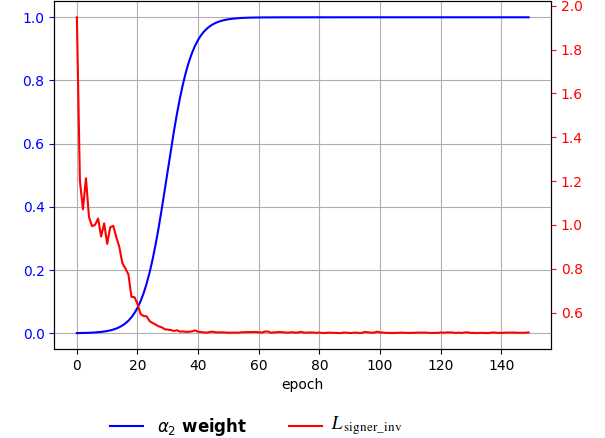
\includegraphics[width=\linewidth]{ChapterFour/desire_signer_inv_loss.png}
        \caption{}
        \label{fig:signer_inv_curve}
    \end{subfigure}
    \hfill
    \begin{subfigure}{0.325\textwidth}
        \centering
        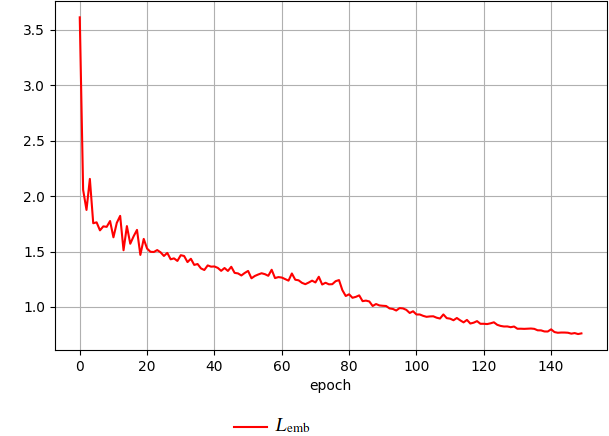
\includegraphics[width=\linewidth]{ChapterFour/desire_emb_loss.png}
        \caption{}
        \label{fig:emb_loss_curve}
    \end{subfigure}
    \hfill
    \begin{subfigure}{0.325\textwidth}
        \centering
        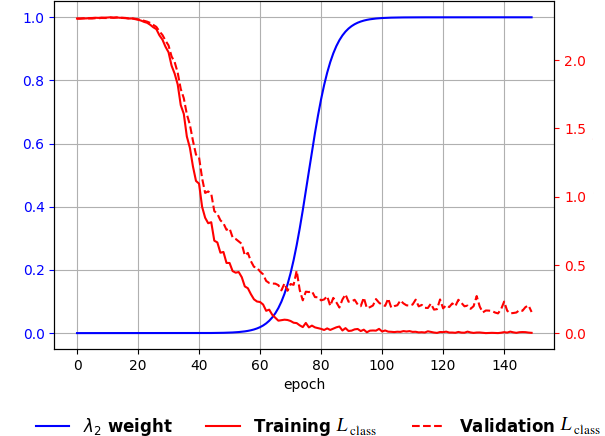
\includegraphics[width=\linewidth]{ChapterFour/desire_class_loss.png}
        \caption{}
        \label{fig:class_loss_curve}
    \end{subfigure}
    \caption{Training behavior of the proposed DeSIRe model: (A) evolution of the $L_{\text{signer\_inv}}$ loss term alongside the corresponding weight $\alpha_{2}$ according to a sigmoid annealing schedule; (B) evolution of the $L_{\text{emb}}$ term value; and (C) evolution of training and validation $L_{\text{class}}$ curves alongside the corresponding weight $\lambda_{2}$ according to a sigmoid annealing schedule.}
    \label{fig:desire_loss_curves}
\end{figure}

\Figref{fig:class_loss_curve} depicts the observed behavior for the classification loss term $L_{\text{class}}$. As previously explained in \Secref{sec:desire_training_strat}, at the start of training, the classification weight $\lambda_{2}$ is set to zero and the $L_{\text{emb}}$ error is backpropagated only through the convolutional block of the classifier module. Therefore, in the first training epochs, $L_{\text{class}}$ remains at a high value, as the classifier predicts random guesses (see \Figref{fig:class_loss_curve}). Then, $L_{\text{class}}$ drops quickly once the classification weight $\lambda_{2}$ starts increasing. This shows that the feature representations learned in the previous phase are highly discriminative for the classification task. On the other hand, the CVAE module starts to be trained on the reconstruction task as soon as the training process begins. At this stage, the sampling scheme associated with the reconstruction loss $L_{\text{rec}}$ is the only mechanism promoting signer-invariance. After a few epochs, the KL weights $\alpha_1$ and $\alpha_2$ start increasing and the CVAE is further enforced to produce signer-invariant latent representations. In particular, \Figref{fig:signer_inv_curve} shows the evolution of the signer-invariance loss $L_{\text{signer\_inv}}$ together with the respective weight $\alpha_2$ and attests that, at the end of training, the encoder produces signer-independent embeddings in the training data. Finally, \Figref{fig:emb_loss_curve} depicts a consistent decrease of the embedding loss $L_{\text{emb}}$ throughout the entire training routine.

\section{Hyperparameter sensitivity analysis}
\label{sec:desire_hyperparams}
This subsection presents a sensitivity analysis of three key hyperparameters of the proposed DeSIRe model, namely the $L_{\text{emb}}$ weight $\lambda_{1}$, the signer-invariance weight $\alpha_{2}$ and the probability of changing the signer identity fed to the decoder network $\rho$. For this purpose, we plotted the curves of the average test accuracy of the proposed model with varying values of $\lambda_{1}\in[0,10]$,  $\alpha_{2}\in[0,10]$, and $\rho\in[0,1]$ (\Figref{fig:desire_hyperparams}). Some interesting conclusions can be drawn from these plots. Particularly, when $\alpha_{1}=0$, $L_{class}$ is the only loss term still active. Accordingly, the proposed DeSIRe model has exactly the same behavior as baseline 1, which results in a significant drop in the test accuracy. When $\lambda_{1}\neq 0$ and $\alpha_{2}=0$, the loss terms $L_{\text{emb}}$, $L_{\text{rec}}$ and $L_{\text{prior}}$ become active and only $L_{\text{signer\_inv}}$ is inactive. Under this setting, the test accuracy increases to $93.75\%$ (see Figure~\ref{fig:desire_hyper_alpha2}). Here, the classifier is trained to follow the latent representations produced by the CVAE. Although the term $L_{\text{signer\_inv}}$ is not present, signer-invariance is still promoted by (i) the $L_{\text{prior}}$ loss term; and (ii) by conditioning the decoder on the signer identity, which is drawn from a random distribution. Finally, when $\lambda_1$ and $\alpha_2$ are both set to their optimal values, all loss terms are active and a maximum test accuracy is achieved. The observed accuracy gain clearly supports the beneficial regularizing effect of the $L_{\text{signer\_inv}}$ loss term, which explicitly promotes signer-invariant representations.

In addition, it is worth mentioning that the proposed DeSIRe model is quite robust to these hyperparameters as the accuracy curves remain quite stable over a large range of values (i.e.\ $\lambda_{1},\alpha_{2}\in [0.01, 1]$). The impact of $\rho$, which controls the proposed sampling scheme of the signer identity in the learning process, is depicted in \Figref{fig:desire_hyper_rho}. From this figure, it is possible to observe that $\rho$ should be set around $0.5$. The test accuracy progressively decreases when $\rho$ falls into the interval $[0.75, 1]$. In these cases, the decoder will be trained most of the time to reconstruct an image of a different signer than the one that was used to produce the encoding. This naturally makes the reconstruction task and the overall CVAE training process too difficult, explaining the noticeable significant performance drop.

\begin{figure*}[t]
    \centering
    \begin{subfigure}{0.325\textwidth}
        \centering
        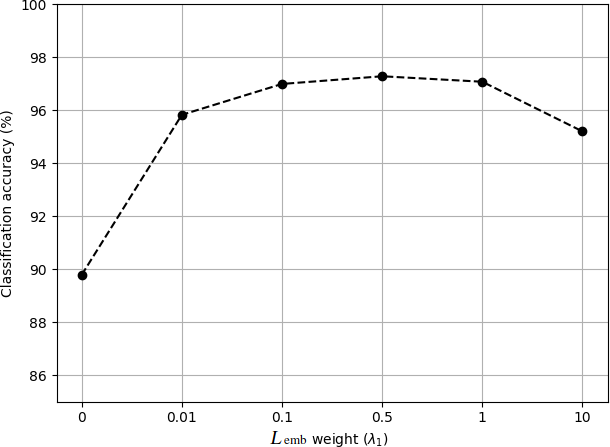
\includegraphics[width=\linewidth]{ChapterFour/desire_hyper_lambda1.png}
        \caption{}
        \label{fig:desire_hyper_lambda1}
    \end{subfigure}
    \hfill
    \begin{subfigure}{0.325\textwidth}
        \centering
        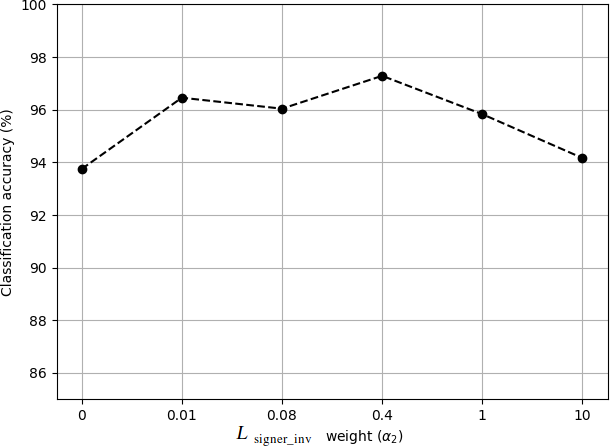
\includegraphics[width=\linewidth]{ChapterFour/desire_hyper_alpha2.png}
        \caption{}
        \label{fig:desire_hyper_alpha2}
    \end{subfigure}
    \hfill
    \begin{subfigure}{0.325\textwidth}
        \centering
        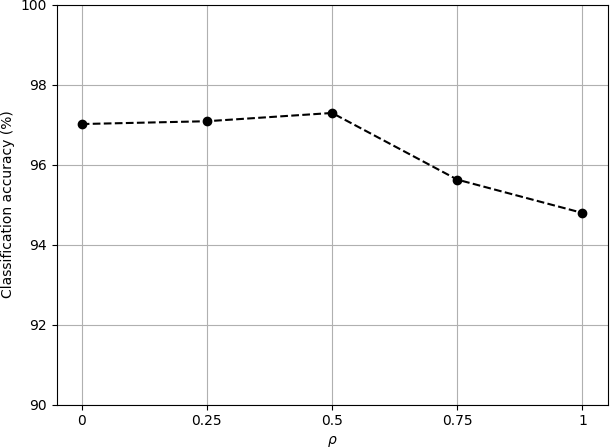
\includegraphics[width=\linewidth]{ChapterFour/desire_hyper_rho.png}
        \caption{}
        \label{fig:desire_hyper_rho}
    \end{subfigure}
    \caption{Hyperparameter sensitivity analysis: (A) The average accuracy of the DeSIRe model with varying values of $\lambda_{1}\in[0,10]$ and $\alpha_{2}=0.4$ and $\rho=0.5$ on the Triesch dataset; (B) The average accuracy of the DeSIRe model with varying values of $\alpha_{2}\in[0,10]$ and $\lambda_{1}=0.5$ and $\rho=0.5$ on the Triesch dataset; and (C) The average accuracy of the DeSIRe model with varying values of $\rho\in[0,1]$ and $\lambda_{1}=0.5$ and $\alpha_{2}=0.4$ on the Triesch dataset.}
    \label{fig:desire_hyperparams}
\end{figure*}
